% Paper 1037, v30 (2026-11-09): built on the collaborator's AnchorMTM_Revised (upstream d67c9c2); see notes/2026-11-09-v30-figure-decisions.md.
% Build: tectonic -X compile --keep-logs method_anchor_figures_updated_en.tex
% Unchanged companion: method_anchor_single_parameter_supplement.tex/.pdf.
% Changes: ANCHORMTM_SINGLE_PARAMETER_VALIDATION.md.
\documentclass[preprint]{vgtc}   % single-blind: authors shown, submission ID in the page header
\usepackage[T1]{fontenc}
\usepackage{mathptmx}
\usepackage{cite}
\usepackage{amsmath,amssymb,amsthm}
\usepackage{placeins}
\usepackage{float,stfloats,needspace}
\usepackage{booktabs,multirow,colortbl}
\makeatletter
\setlength{\@dblfptop}{0pt}
\setlength{\@dblfpsep}{12pt}
\setlength{\@dblfpbot}{0pt plus 1fil}
\makeatother
\usepackage[ruled,vlined]{algorithm2e}
\SetKwInput{KwData}{Data}
\SetKwInput{KwResult}{Result}
\SetKwProg{Fn}{Function}{:}{}
\SetKw{KwReturn}{return}
\SetKw{KwBreak}{break}
\SetKwFunction{Construct}{ConstructTemporalMap}
\SetKwFunction{Refine}{RefineOrder}
\SetKwFunction{Barriers}{OptimalBarriers}
\SetAlFnt{\small}
\SetAlCapFnt{\small\bfseries}
\SetAlCapNameFnt{\small\bfseries}
\SetAlCapSkip{3pt}
\DontPrintSemicolon
\setcounter{secnumdepth}{3}
\newtheorem{theorem}{Theorem}
\newtheorem{lemma}{Lemma}
\newtheorem{proposition}{Proposition}
\newcommand{\dtop}{d_{\mathrm{top}}}
\newcommand{\lca}{\operatorname{lca}}
\newcommand{\nroe}{\mathrm{NROE}}
\newcommand{\pos}[1]{\left[#1\right]^+}
\title{AnchorMTM: Spatially Anchored Merge Tree Maps\\for Time-Varying Scalar Fields}
\author{%
Lele~Wang$^{1,2}$\thanks{%
Affiliations:
$^{1}$ Advanced Interactive Technology and Application Laboratory, Computer Network Information Center, Chinese Academy of Sciences, Beijing, China;
$^{2}$ University of Chinese Academy of Sciences, Beijing, China;
$^{3}$ Hangzhou Institute for Advanced Study, UCAS, Hangzhou, China.
E-mails: lelewang@cnic.cn; dongyu@cnic.cn; yxmeng@cnic.cn;
liguan@sccas.cn; wangzhe@sccas.cn; sgh@sccas.cn;
liujun@sccas.cn.
Lele Wang and Yu Dong contributed equally to this work.
Jun Liu is the corresponding author.}%
\quad
Yu~Dong$^{1,*}$%
\quad
Yuxiang~Meng$^{1,2}$%
\quad
Guan~Li$^{1,2}$%
\quad
Zhe~Wang$^{1,2}$%
\quad
Guihua~Shan$^{1,2,3}$%
\quad
Jun~Liu$^{1,2}$\thanks{Corresponding author. E-mail: liujun@sccas.cn.}
}
\preprinttext{Online Submission ID: 1037}
\onlineid{1037}
\vgtccategory{Research}
\vgtcinsertpkg
\usepackage{tikz}
\hypersetup{pdftitle={AnchorMTM: Spatially Anchored Merge Tree Maps for Time-Varying Scalar Fields},pdfauthor={Lele Wang, Yu Dong, Yuxiang Meng, Guan Li, Zhe Wang, Guihua Shan, Jun Liu}}
\abstract{Temporal merge tree maps summarize the hierarchy of a time-varying scalar field, but their display coordinate does not provide a fixed spatial reference. Anchoring this coordinate reveals a structural conflict: exact topology requires contiguous subtree blocks, whereas projected feature positions can interleave. We quantify the resulting positional cost through three layout-independent bounds for exact point orders, finite-width interval layouts and bounded merge-level error. AnchorMTM uses these bounds to guide leaf-order selection and capped anchor placement, then reconstructs scalar profiles under a controlled merge budget. Controlled four-leaf experiments compare the bounds with exhaustive ordering and independent linear programs. Existing results on five planar and two volumetric sequences then connect unavoidable displacement, absolute positioning and the effect of relaxation. The per-frame evidence shows that a budget resolves a difficult tail of Storms frames and shifts most frames in the default volume configurations. The resulting maps make feature positions readable against one shared spatial direction while exposing the hierarchical cost of that coordinate.}
\keywords{Time-varying scalar fields, merge tree maps, spatial anchoring, topology preservation, constrained layout.}
\teaser{
\centering
\begin{tikzpicture}
\node[anchor=south west,inner sep=0] (img) at (0,0) {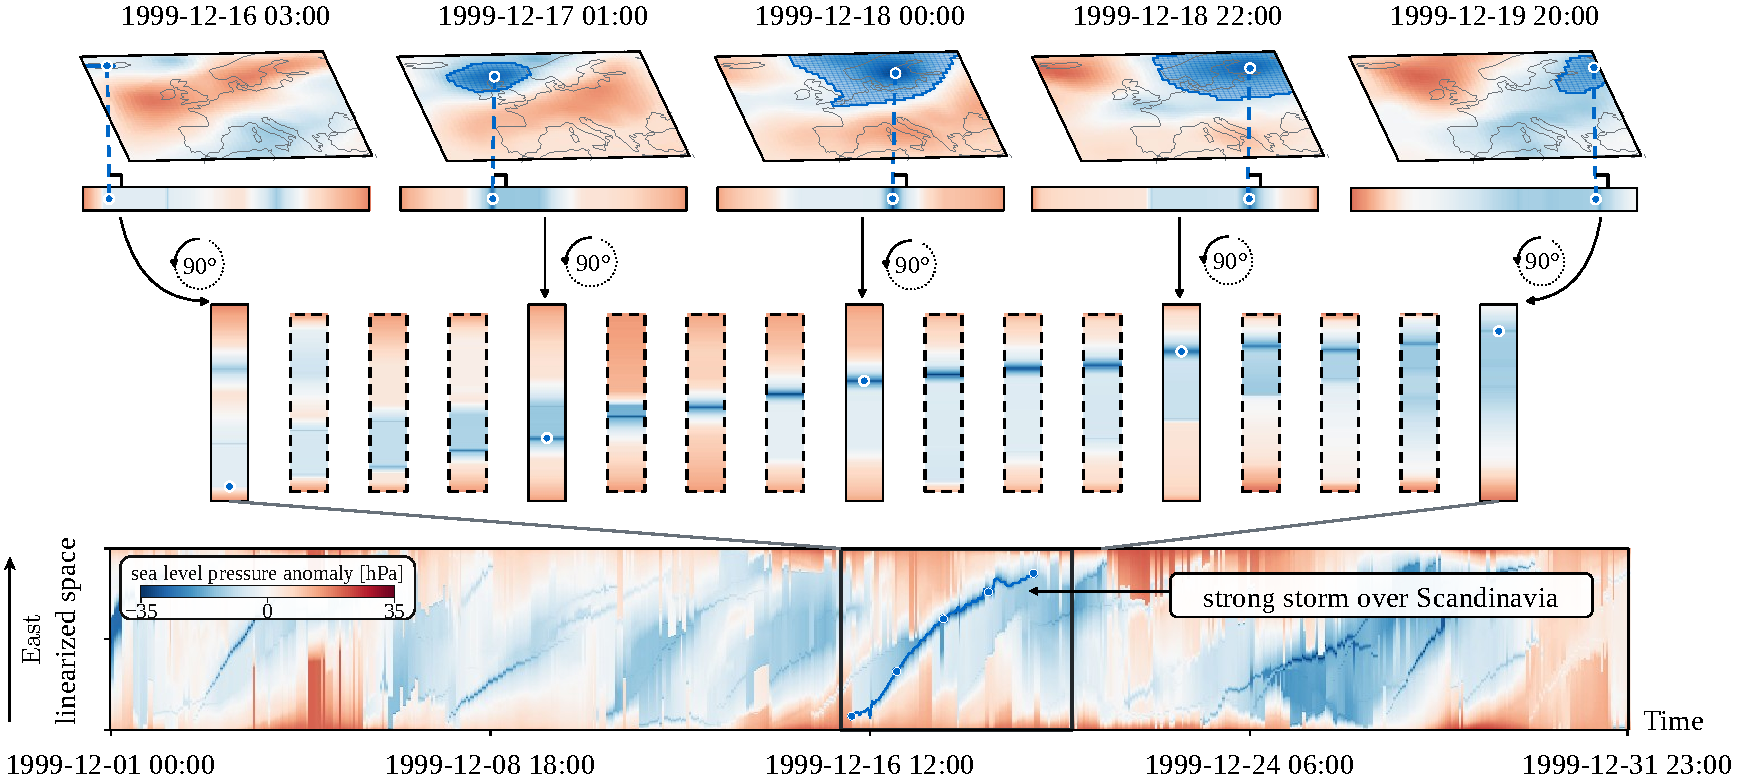
\includegraphics[width=\linewidth]{figures/anchor_storms_overview.pdf}};
\begin{scope}[x={(img.south east)},y={(img.north west)}]
\draw[-{latex},line width=0.9pt,black!80] (0.94,0.13) -- (0.94,0.325);
\node[font=\footnotesize\rmfamily,anchor=west,inner sep=1pt] at (0.947,0.14) {W};
\node[font=\footnotesize\rmfamily,anchor=west,inner sep=1pt] at (0.947,0.315) {E};
\node[font=\footnotesize\rmfamily,anchor=west,inner sep=1pt] at (0.947,0.2275) {$a^*$};
\end{scope}
\end{tikzpicture}
\par
\refstepcounter{figure}\label{fig:storms_overview}
{\captionfonts\raggedright\noindent\figurename~\thefigure: Storms temporal overview ($\varepsilon=5\%$): 744 hourly ERA5 sea-level-pressure fields, December 1999. Each frame's merge tree becomes a one-dimensional profile, rotated and stacked along time. The vertical axis is one fixed spatial direction $a^*$ (arrow, west to east), so the rising track is a storm moving east, from the open Atlantic to Scandinavia; the snapshots identify the matched extremum, and blue outlines show its leaf-arc support. The map keeps every nesting and merge level within the 5\% budget.\par}

}
\linespread{1.0}
\setlength{\textfloatsep}{7pt}
\setlength{\floatsep}{6pt}
\setlength{\dbltextfloatsep}{7pt}
\setcounter{dbltopnumber}{2}
\renewcommand{\dbltopfraction}{0.9}
\renewcommand{\dblfloatpagefraction}{0.7}
\renewcommand{\floatpagefraction}{0.7}
\setcounter{totalnumber}{6}
\setcounter{topnumber}{3}
\setcounter{bottomnumber}{3}
\renewcommand{\textfraction}{0.07}

\newcommand{\paperfigure}[4][\textwidth]{\centering\includegraphics[width=#1]{#2}\caption{#4}\label{#3}}


\begin{document}
\firstsection{Introduction}
\maketitle
\raggedbottom
\setlength{\emergencystretch}{1.5em}
Time-varying scalar fields record how quantities such as sea-level pressure, aerosol concentration or vorticity evolve over a spatial domain. Analysts study them through features, such as low-pressure systems, pollution episodes or shed vortices, and ask three questions about each: how it relates to the others, where it is, and how it moves. Animation keeps every time step in its spatial context but makes distant times hard to compare~\cite{Tversky:2002:Animation,Robertson:2008:Animation}. Static overviews therefore assign one display axis to time and compress space into the other, so that a whole sequence fits into one image~\cite{Bach:2017:STC}. What that second axis means decides which of the three questions the overview can answer. The Hovm\"oller diagram of atmospheric science keeps a physical coordinate such as longitude and shows an eastward-moving system as a slanted streak~\cite{Hovmoller:1949}, but it averages the field over the remaining coordinates, so neighboring features blend and their hierarchy disappears.

Merge tree maps answer the first question. A merge tree records how sublevel sets connect as the threshold rises: its leaves are the extrema, and its internal nodes are the levels at which regions merge~\cite{Heine:2016:Survey,Edelsbrunner:2002:TPS}. Temporal merge tree maps (TMTM) draw the tree of each time step as a one-dimensional profile whose minima are the extrema and whose barriers are the merge levels, and they stack the profiles into one image~\cite{Koepp:2023:TMTM}. Spatiotemporal merge tree maps (ST-MTM) additionally arrange the features by their pairwise distances and temporal coherence~\cite{STMTM:2026}. In both, the vertical axis follows the tree, temporal alignment or relative distance; neither fixes an origin or a direction in space. A storm that crosses the North Atlantic within a few days can therefore stay at the same height of the map, and the reader sees how it connects to neighboring lows but not where it is or which way it moves.

We give this axis a spatial meaning. Fixing one direction $a^*$ in the domain assigns every extremum a reference position, the projection of its location onto $a^*$, and a map whose axis encodes location should draw each extremum at its reference (Fig.~\ref{fig:storms_overview}). The obstacle is the tree itself. A profile shows the tree exactly only if every subtree occupies one contiguous block of leaves, but the references of two sibling subtrees may interleave (Fig.~\ref{fig:related-work-mapping}d). No exact profile can then place every feature at its reference, whatever algorithm draws it. This conflict raises three questions: how much displacement the tree forces, where in the tree this displacement arises, and how much merge-level fidelity must be given up to remove it. Without answers, the positional error of a map cannot be attributed to the data or to its layout, and an analyst cannot judge whether a spatial axis is worth its cost.

We answer these questions with bounds and turn the answers into a construction. Three lower bounds, for exact topology, for features of finite width and for a bounded merge error, depend only on the trees, the references and the widths, so the positional price of the axis is known before any layout is computed and applies to every map that keeps the tree. AnchorMTM then computes the map directly from the field sequence and one merge budget $\varepsilon$. It searches leaf orders that the budget admits, using a closed-form test for the smallest merge error an order can show, places the extrema as close to their references as the chosen order allows, and reconstructs the profiles. With $\varepsilon=0$, the map shows every tree exactly; with $\varepsilon>0$, it releases the conflicts that a small change of merge levels can resolve and records the merge error each frame actually spends.

Our contributions are as follows.
\begin{itemize}\setlength{\itemsep}{1pt}\setlength{\parsep}{0pt}
\item We formulate spatially anchored merge tree maps and derive three layout-independent lower bounds on the displacement that keeping the tree forces, for exact topology, finite widths and bounded merge error. The bounds locate the conflict in the tree and measure any merge tree map, including existing ones.
\item We present AnchorMTM, which builds the leaf order and extremum positions of every frame from the projected locations, so that the height of a band reads as location and its drift as motion along $a^*$, while the profile keeps the nesting and merge levels of the tree. A merge budget $\varepsilon$, enforced through optimal merge barriers and checked on every rendered frame, controls how much merge-level fidelity may be traded for position.
\item On five planar and two volumetric sequences, we show that the bounds are tight on controlled and real trees, that most of the order error of existing maps is not forced by the tree, and how a budget reshapes the displacement of individual frames.
\end{itemize}

\section{Related Work}\label{sec:related}
\subsection{Linearizing Space for Temporal Overviews}
Animation preserves the spatial context of each time step, whereas static overviews let viewers compare distant times directly; which serves better depends on the task~\cite{Tversky:2002:Animation,Robertson:2008:Animation}. Bach et al.\ describe both, and the operations between them, as transformations of a space--time cube~\cite{Bach:2017:STC}. A static overview must linearize space, and Fig.~\ref{fig:related-work-mapping} contrasts three ways to do so. \emph{Domain-based} linearizations traverse the samples: Hovm\"oller diagrams keep one physical coordinate and average over the others~\cite{Hovmoller:1949}, while geographic orderings, dense pixel displays and space-filling curves visit the whole domain~\cite{Guo:2006:SpatialOrder,Dafner:2000:CSFC,Rauscher:2025:1DO}, and volume lines and data-driven curves extend such traversals to volumes~\cite{Weissenboeck:2019:DVL,Zhou:2021:DSF}. \emph{Feature-based} summaries order selected entities: one-dimensional projections, MotionRugs, stable visual summaries and MoReVis rank moving objects by position or stability~\cite{Franke:2021:1DP,Buchmueller:2019:MR,Wulms:2021:SVS,Valdrighi:2024:MRV}. Every linearization distorts some spatial relations~\cite{Nonato:2019:MP,Aupetit:2007:VD}. These overviews keep a spatial coordinate but no feature hierarchy; AnchorMTM keeps the merge tree and makes explicit what a spatial coordinate then costs.

\begin{figure}[!tb]
\centering
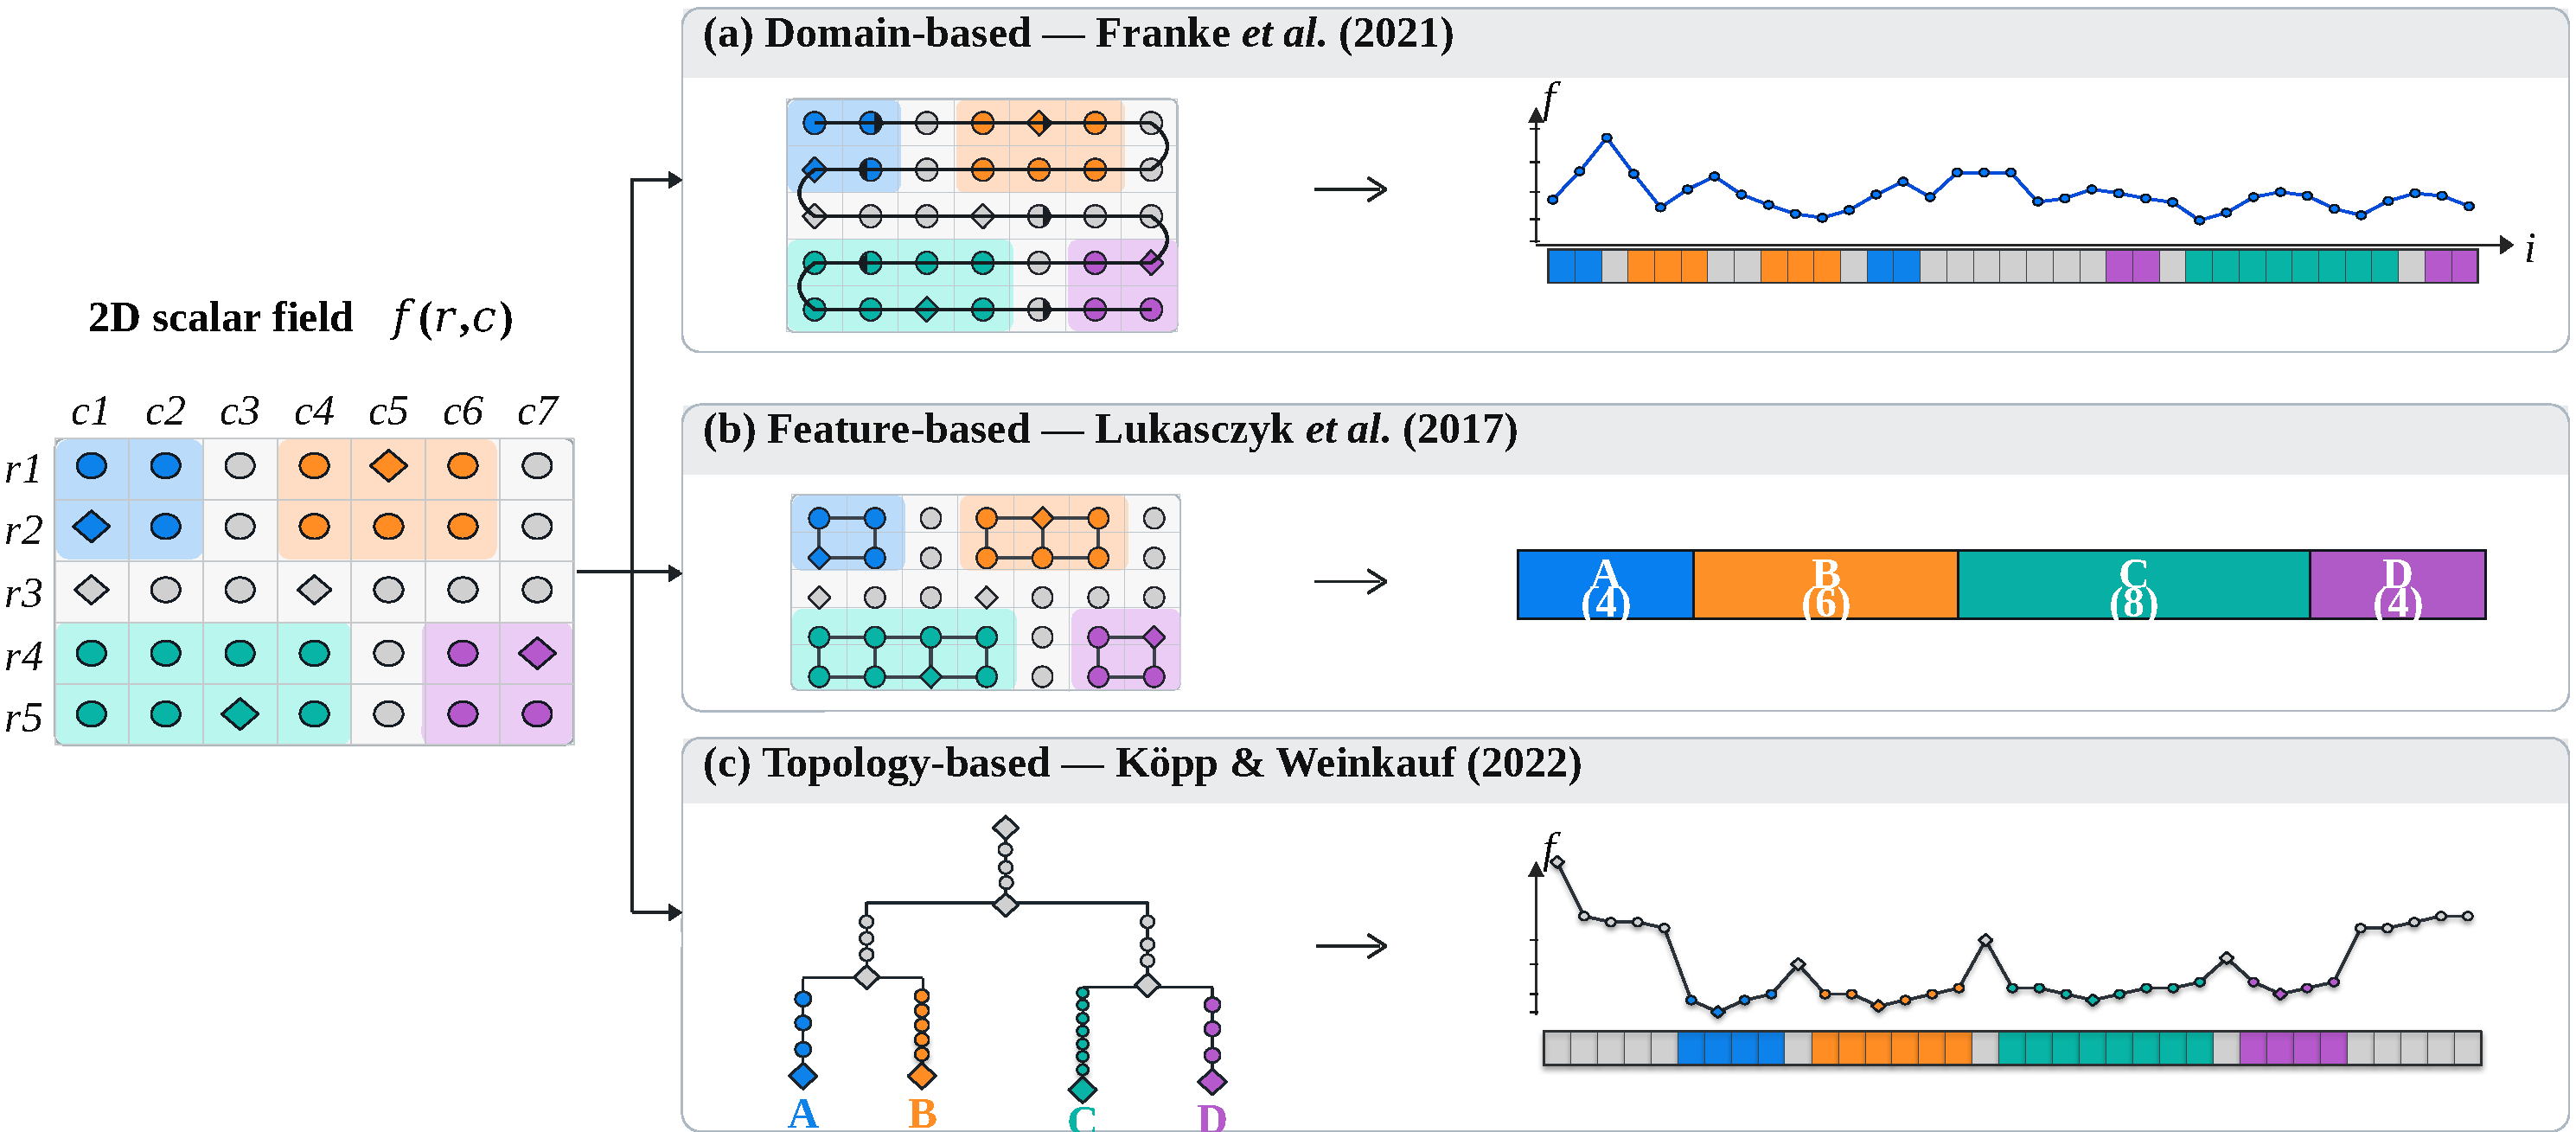
\includegraphics[width=\columnwidth]{figures/anchor_related_work_mapping.pdf}\\[2pt]
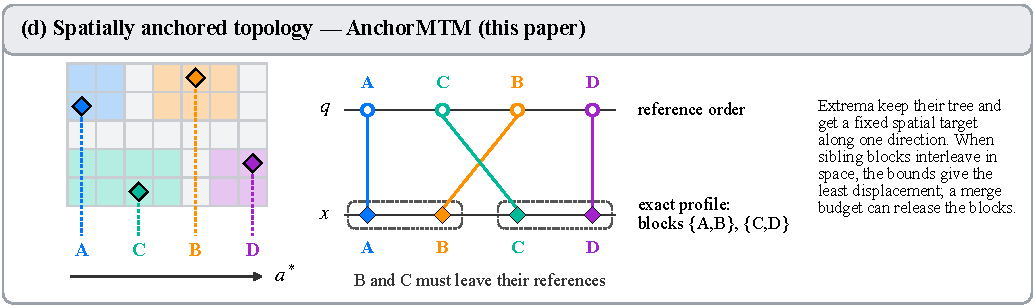
\includegraphics[width=\columnwidth]{figures/anchor_related_work_panel_d.pdf}
\caption{Mapping strategies on a common 35-sample field. (a) Domain traversal keeps samples; (b) a 22-sample feature summary keeps selected structures; (c) a topology-based profile keeps the hierarchy, but its axis has no spatial meaning. (d) AnchorMTM keeps the hierarchy and gives every extremum a target along one direction $a^*$; here the targets interleave the subtree blocks $\{A,B\}$ and $\{C,D\}$, the conflict that Sections~\ref{sec:bounds} and~\ref{sec:method} quantify and resolve.}
\label{fig:related-work-mapping}
\end{figure}
\subsection{Topology of Time-Varying Scalar Fields}
Merge trees and contour trees summarize how level sets connect, and persistence-based simplification controls their size~\cite{Heine:2016:Survey,Edelsbrunner:2002:TPS,Tierny:2018:TTK}. Features are tracked over time by region overlap or attribute similarity~\cite{Silver:1997:Tracking,Saikia:2017:GFT} and shown as tracking graphs and nested tracking graphs~\cite{Widanagamaachchi:2012:DTG,Lukasczyk:2017:NTG,Lukasczyk:2020:DNTG}. Time-varying merge trees have been computed and compared with Wasserstein and geometry-aware interleaving distances~\cite{Oesterling:2017:TVMT,Pont:2022:WMT,Yan:2022:GAMT,Yan:2021:Survey}, and such pipelines follow tropical cyclones and atmospheric rivers~\cite{Yan:2024:TROPHY,Lan:2024:AR}. The merge error we budget is a labelled cophenetic discrepancy that equals the labelled interleaving distance~\cite{Munch:2019:LINF,Gasparovic:2024:IID,Morozov:2013:IDMT} and relates to distances between ordered merge trees~\cite{Beurskens:2025:OMT}. Tracking graphs show how features appear, split and merge, but not where they are; merge tree maps additionally show the values and nesting of every time step, and AnchorMTM adds their location.

\subsection{Drawing Hierarchies along One Axis}
Topological landscapes draw a merge tree as a terrain or as a one-dimensional profile whose minima are the extrema and whose barriers are the merge levels~\cite{Weber:2007:TL,Oesterling:2013:TLP}; geometry-preserving and temporally coherent variants exist~\cite{Beketayev:2012:GPTL,Herick:2020:TCTL}, and contour trees have been drawn in the plane and in joint layouts~\cite{Heine:2011:DCT,Lohfink:2020:FCT}. Temporal treemaps lay out evolving hierarchies along time~\cite{Koepp:2019:TT}. TMTM aligns the profiles of successive merge trees into one static map~\cite{Koepp:2023:TMTM}, and ST-MTM adds relative spatial distances and temporal stability~\cite{STMTM:2026}; their axes encode tree traversal or relative distance. Storyline layouts face a related problem for groups of entities and balance crossings and wiggles against group contiguity~\cite{Tanahashi:2012:Storyline,Liu:2013:SF}.

The conflict we study arises whenever a hierarchy must respect an external order. Optimal leaf ordering selects a tree-consistent order of a dendrogram that keeps similar leaves adjacent~\cite{BarJoseph:2001:OLO,Eisen:1998:CA}, and tree reordering seeks the tree-consistent permutation closest to a target order~\cite{Bulteau:2022:RT}. Spatially ordered treemaps and data--spatial grid maps trade hierarchy or data layout against geographic position~\cite{Wood:2008:SOT,vanBeusekom:2023:DSL}, geophylogenies connect leaf orders to map locations~\cite{Klawitter:2025:GP}, and tanglegram layouts minimize crossings or displacement between two trees~\cite{Fernau:2010:CTC,Huson:2026:DOT}. Separation constraints keep laid-out objects disjoint~\cite{Dwyer:2006:IPSEP,Li:2019:SOI}, minimax ultrametric fitting is closely related to our optimal barriers~\cite{Farach:1995:RM}, and merge distortion and topology-preserving projections measure how much hierarchy a mapping retains~\cite{Eldridge:2015:MD,Doraiswamy:2021:TM}. These methods optimize crossings, sums or stress for a given instance. We instead bound, in closed form for points, the worst displacement that every tree-consistent layout must accept, together with the merge error that removes it.

\section{Problem Formulation}\label{sec:formulation}\label{sec:background}
\subsection{Merge Trees, Profiles, and Feature Identity}
For a sampled field $f_t$, the merge tree $T_t$ records sublevel components created at minima and joined at saddles; negating the field handles maxima~\cite{Tierny:2018:TTK}. Extraction and persistence simplification precede layout. A leaf $i$ has extremum location $p_i^t$ and support $S_i^t$, comprising the samples on its leaf arc. Augmented internal arcs retain samples for filling the profile (Supplementary Fig.~S2). Write $h_t(v)$ for a node's scalar level and $\mathcal{D}_t(v)$ for its descendant leaves. The fixed-label merge matrix is
\begin{equation}\label{eq:merge}
V_{ij}^t=h_t(\lca(i,j)),\quad i\ne j;\qquad V_{ii}^t=f_t(p_i^t).
\end{equation}
Equal-level merges form one multifurcation. A one-dimensional profile $\psi_t$ places the extrema in leaf order $\pi_t$; the largest profile value between anchors $i,j$ gives their displayed merge level $V_{ij}^{\psi_t}$. We call a profile \emph{exact} if every displayed merge level equals that of the tree; this requires the leaves of every subtree to form one contiguous block.

On a fixed grid, one-to-one Hungarian matching maximizes $|S_i^{t-1}\cap S_j^t|$ and discards zero-overlap pairs~\cite{STMTM:2026}; a matched leaf inherits its track identity, and $\mu_t(i)$ denotes its predecessor. These links supply the temporal targets and the motion samples below, and the same matching is reused for every budget (Supplementary Fig.~S3).

\subsection{Fixed Spatial Reference}\label{sec:reference-model}
The default direction maximizes squared matched-extremum motion:
\begin{equation}\label{eq:autodirection}
a^*\in\arg\max_{\|a\|=1}a^\top\Bigl(\sum_{t,i}\Delta p_i^t(\Delta p_i^t)^\top\Bigr)a,
\end{equation}
where $\Delta p_i^t=p_i^t-p_{\mu_t(i)}^{t-1}$ over valid links. Its sign makes total projected motion nonnegative; the longest domain axis handles zero motion energy. An analyst may supply a physical direction instead. This separates reference estimation from the layout search: a budget changes the admissible map, while the coordinate being approximated stays fixed. Projected domain corners define one origin $o$ and extent $L$, giving
\begin{equation}\label{eq:reference}
q_i^t=\langle a^*,p_i^t\rangle-o\in[0,L].
\end{equation}
Direction, origin and extent remain fixed across frames and budgets. Relative geometry uses support-centroid distances $d_{ij}^t$; the targets $q_i^t$ use extremum locations. Thus support growth can change relative-distance terms without moving a feature's spatial target.

\subsection{A Unified Layout Formulation}\label{sec:common}
Each leaf occupies an interval of width $W_i=s\,m_i$ and center $z_i$, where $m_i$ is its support measure and $s$ is fixed. The layout set $\mathcal{L}(\pi;W)$ places these intervals in order $\pi$ inside $[0,L]$, with gap at least $g$ and anchor slack $|x_i-z_i|\le\rho W_i/2$. Two order costs distinguish point ordering from packing, and NPE measures the drawn map:
\begin{equation}\label{eq:nroe}
\begin{aligned}
\nroe(\pi)&=\frac{\max_{j\le k}[q_{\pi(j)}-q_{\pi(k)}]^+}{2L},\\
\tau(\pi)&=\min_{(x,z)\in\mathcal{L}(\pi;W)}\|x-q\|_\infty ,\\
\mathrm{NPE}&=\frac1T\sum_{t}\frac{\|x^t-q^t\|_\infty}{L}.
\end{aligned}
\end{equation}
The normalized reference-order error NROE is the smallest worst displacement, relative to the axis length, of point anchors kept in order $\pi$; we call it the \emph{order error} of $\pi$. The fixed-order cost $\tau$ adds the intervals; it is the optimum of a minimax linear program and has a closed form (Supplementary Section~S1). The normalized position error NPE, which we propose here, is the worst displacement a drawn map actually has, relative to the axis length and averaged over frames. It takes the worst displacement of a frame because that is what the bounds of Section~\ref{sec:bounds} constrain, so the two can be compared directly. The merge error measures how far the displayed hierarchy departs from the tree:
\begin{equation}\label{eq:dtop}
\dtop(\psi,T)=\max_{i,j}|V_{ij}^{\psi}-V_{ij}|.
\end{equation}
The diagonal includes extremum values. Under complete fixed labelling this cophenetic error equals the labelled interleaving distance and bounds the unlabelled interleaving and bottleneck distances~\cite{Munch:2019:LINF,Gasparovic:2024:IID,Morozov:2013:IDMT}.

These variables separate layout priorities in the common model
\begin{equation}\label{eq:family}
\begin{aligned}
\min_{\pi\in\Pi,\,(x,z)\in\mathcal{L}(\pi;W)}\;&\lambda_RE_R+\lambda_GE_G+\lambda_ME_M+\lambda_CE_C\\
\mathrm{s.t.}\;&\dtop\le\eta.
\end{aligned}
\end{equation}
Each term is a mean squared residual over the $n_t$ leaves, the ordered pairs $P_t$ or the matched leaves $M_t$ of a frame:
\begin{equation}\label{eq:terms}
\begin{aligned}
E_R&=\tfrac{1}{n_t}\textstyle\sum_i(x_i-q_i)^2, & E_G&=\tfrac{1}{|P_t|}\textstyle\sum_{(i,j)\in P_t}(x_j-x_i-d_{ij})^2,\\
E_M&=\tfrac{1}{|M_t|}\textstyle\sum_{i\in M_t}(x_i-\hat x_i)^2, & E_C&=\tfrac{1}{n_t}\textstyle\sum_i(x_i-z_i)^2,
\end{aligned}
\end{equation}
with the temporal target $\hat x_i$ of Section~\ref{sec:method}. The allowance $\eta$, in scalar units, makes the tradeoff explicit: $\eta=0$ demands the exact tree, and a larger $\eta$ admits orders that follow the references more closely. Section~\ref{sec:method} sets $\eta$ from a merge budget $\varepsilon$ given as a fraction of the scalar range. TMTM packs tree-compatible blocks and aligns them by overlap, so its layout follows from the leaf order alone; ST-MTM fits relative geometry with temporal constraints, which corresponds to $\lambda_R=0$ and a stationary temporal target. Both keep the tree ($\eta=0$) and have no reference term, so nothing ties their axes to location. AnchorMTM adds $E_R$ and a declared allowance. It does not solve Eq.~\ref{eq:family} jointly: it first chooses the leaf order and then solves a capped quadratic program for the anchors (Section~\ref{sec:method}). Eq.~\ref{eq:family} states what each method optimizes; it does not rank them. A setting that gives position the largest weight is not expected to match, on relative distances, a method that optimizes only those.

\subsection{Conflict Between Topology and Spatial Position}
A projection can follow every $q_i$, but a profile that shows the tree exactly must keep each subtree in one block. In the exact panel of Fig.~\ref{fig:framework}, the tree joins $A$ with $B$ and $C$ with $D$, while the references occur in the order $A,C,D,B$: block $\{C,D\}$ lies inside the span of block $\{A,B\}$, so some extrema must leave their references. Keeping the blocks displaces anchors; allowing some merge error may admit an order closer to the references. How far the anchors must move depends only on the tree, the references, the widths and the allowance, not on the algorithm that draws the map.

We address three questions: how much displacement exact topology forces (RQ1), how finite feature widths and interval constraints increase that cost (RQ2), and which conflicts can be released by bounded merge-level error (RQ3). The next section answers them in this order; the construction then uses the same quantities to select and place a map.

\section{The Positional Price of Keeping the Tree}\label{sec:bounds}
The positional cost comes from two sources: constraints imposed by the hierarchy and additional choices made by a layout. We first isolate the hierarchy in a point model, then account for interval packing, and finally allow a bounded merge error. This progression answers RQ1--RQ3 using the same reference coordinate. Suppress $t$, write $[v]^+=\max(v,0)$ and take empty maxima as zero; the proofs are in Supplementary Section~S2.

\subsection{Exact Topology}
The first question removes feature width and asks what the hierarchy alone forces. An exact profile keeps sibling subtrees in separate blocks, so their reference hulls determine the cost of either block orientation. Let $[m_X,M_X]$ be the reference hull of subtree $X$, the smallest interval that contains the references of its leaves.
\begin{proposition}[Exact-topology bound]\label{thm:order}
Every exact profile satisfies $\nroe(\pi)\ge\nu^*$, where
\begin{equation}\label{eq:nu}
\nu^*=\frac{1}{2L}\max_v\max_{X\ne Y\in\mathrm{ch}(v)}[\min(M_X-m_Y,M_Y-m_X)]^+.
\end{equation}
Ordering the children of every node by the midpoints of their hulls attains $\nu^*$ in $O(n\log n)$ time.
\end{proposition}
Two sibling blocks must take one orientation, and each orientation inverts some references: placing $X$ first costs $[M_X-m_Y]^+/2$, placing $Y$ first $[M_Y-m_X]^+/2$, and midpoint order chooses the smaller. Every inverted pair of leaves is separated at its lowest common ancestor, so the midpoint order has no larger inversion. Any order error above $\nu^*$ is therefore chosen by the layout, not forced by the tree; we call it \emph{not forced}.

\subsection{Finite Widths}
Set $H_i=\rho W_i/2$, $\ell_i=q_i-W_i/2-H_i$, $r_i=q_i+W_i/2+H_i$ and $s_i=W_i+g$. For a set $S$ of leaves, the packing summaries
\begin{equation}\label{eq:packing}
\begin{split}
A(S)&=\max_{a\in S}\bigl(\ell_a+\sum_{i\in S:\ell_i\ge\ell_a}s_i\bigr),\\
B(S)&=\max_{b\in S}\bigl(\sum_{i\in S:r_i\le r_b}s_i-r_b\bigr)
\end{split}
\end{equation}
bound how far right the intervals of $S$ must reach and, negated, how far left they must begin, given their references and anchor slack. Define $\omega(X,Y)=\tfrac12\min\{A(X)+B(Y),A(Y)+B(X)\}-g/2$ for two disjoint leaf sets, and the canvas term $E_\partial=\max\{0,B(\mathcal F)-g,A(\mathcal F)-g-L\}$ for the set $\mathcal F$ of all leaves.
\begin{proposition}[Width-aware bound]\label{thm:width}
For every exact interval layout in order $\pi$,
\begin{equation}\label{eq:widthbound}
\|x-q\|_\infty\ge\tau(\pi)\ge\mathcal B_w
=\max\{E_\partial,\max_{(X,Y)\in\mathcal P_0}\omega(X,Y)\},
\end{equation}
where $\mathcal P_0$ is the set of pairs of sibling subtrees, taken as leaf sets. With zero widths and gaps, $\mathcal B_w=L\nu^*$.
\end{proposition}
The first and last anchors of a block must enclose its intervals and gaps, up to the anchor slack, and the two canvas ends add $E_\partial$. Ordering alone therefore no longer determines the positional cost: even an order that attains the point bound may need further displacement to fit its intervals. $\mathcal B_w$ is in coordinate units, whereas $\nu^*$ is normalized by $L$. The construction therefore evaluates the exact packing cost $\tau$ of each candidate order before it places the anchors.

\subsection{Bounded Merge Error}
In a profile with $\dtop\le\eta$, if leaf $k$ lies between descendants $i,j$ of node $u$, the interval between $i$ and $k$ lies inside that between $i$ and $j$, so $V_{ik}^{\psi}\le V_{ij}^{\psi}$ and hence $V_{ik}\le h(u)+2\eta$. Let $\mathrm{Anc}_\eta(u)$ be the highest ancestor of $u$ with $h(\mathrm{Anc}_\eta(u))-h(u)\le2\eta$. Form $\mathcal P_\eta$ from the pairs $(\mathcal D(u),\{k\})$ with $k\notin\mathcal D(\mathrm{Anc}_\eta(u))$, and the pairs $(\mathcal D(u),\mathcal D(w))$ of internal nodes $u,w$ in which each set is disjoint from the other's $\mathcal D(\mathrm{Anc}_\eta(\cdot))$.
\begin{proposition}[Bounded-merge-error bound]\label{thm:chain}
If $\dtop\le\eta$, then for every pair $(X,Y)\in\mathcal P_\eta$ the leaves of $X$ all precede or all follow those of $Y$. Thus
\begin{equation}\label{eq:chainbounds}
\begin{split}
\nroe(\pi)&\ge C_\eta=\max_{(X,Y)\in\mathcal P_\eta}\frac{[\min(M_X-m_Y,M_Y-m_X)]^+}{2L},\\
\tau(\pi)&\ge C_{w,\eta}=\max\{E_\partial,\max_{(X,Y)\in\mathcal P_\eta}\omega(X,Y)\}.
\end{split}
\end{equation}
\end{proposition}
The test uses the accumulated level difference to the ancestor, so an allowance releases only the conflicts between subtrees that merge within $2\eta$ of each other. Flattening every node whose parent lies at most $2\eta$ above it and applying Propositions~\ref{thm:order} and~\ref{thm:width} to the flattened tree gives a second valid bound; neither dominates, and we report the larger. Together, the three bounds separate displacement forced by the tree from displacement chosen by a layout. They also suggest the construction: search orders by their exact fixed-order cost $\tau$, admit an order only when its merge error fits the allowance, and limit further displacement when placing the anchors. A lower bound does not produce a map; the construction must still build one and check it.

\begin{figure*}[!tb]
\paperfigure{figures/anchor_framework.pdf}{fig:framework}{AnchorMTM workflow on a four-leaf example. Extract and reference: merge trees of the input frames $F(x,t)$, leaf supports matched across frames, and one direction $a^*$ that gives every extremum a reference position $q$; the bounds follow from these quantities alone. Topology-budgeted layout: with $\varepsilon=0$ the leaf order keeps every subtree contiguous and the anchors $x$ leave their references; with $\varepsilon>0$ a relaxation candidate admits an order that follows them, and the anchors are placed under a displacement cap. Linearized space: leaf-arc samples and optimal barriers fill each profile $\psi_t$, every rendered frame is checked against the budget, and the stacked profiles form the map.}
\end{figure*}
\section{The AnchorMTM Method}\label{sec:method}\label{sec:construction}

Figure~\ref{fig:framework} summarizes the method. \emph{Extract \& reference} prepares the trees, identities and fixed targets defined in Section~\ref{sec:formulation}. \emph{Topology-budgeted layout} first chooses an admissible leaf order with low $\tau$ and then places the anchors, balancing spatial and temporal objectives within a cap on that order's displacement. \emph{Linearized space} builds the scalar profiles and stacks them along time. The output of each stage fixes the constraints passed to the next. The control is a normalized merge allowance $\varepsilon$, with $\eta=(\varepsilon_0+\varepsilon)\Delta_F$ for sequence scalar range $\Delta_F$ and numerical tolerance $\varepsilon_0=10^{-7}$. Exact sets $\varepsilon=0$, so merge levels closer than $2\varepsilon_0\Delta_F$ count as equal; this matters only on Cylinder, where Exact then has merge error $10^{-7}$ of the range with respect to the original tree and NPE 9.2\%, against 13.6\% with these levels kept distinct (Supplementary Section~S4.11). A budgeted map uses a positive allowance, and Balanced denotes one experimentally selected budget, not all budgeted maps. Widths, gap, slack and weights stay fixed during a budget sweep; the merge allowance controls hierarchical error rather than directly bounding positional error.

\subsection{Order Selection and Optimal Barriers}
Order search receives the prepared tree, reference targets, widths and merge allowance. A finite candidate pool $\mathcal C$ starts from midpoint orders of the strict tree, threshold flattenings and selective conflict flattenings. Width-aware block moves refine promising structures (Supplementary Section~S3). The point bound supplies an exact-topology initialization, and the interval analysis is why candidates are ranked by their packing cost $\tau$. Each visited order is checked against the original merge matrix, and selection is lexicographic:
\begin{equation}\label{eq:orderobjective}
\pi^\varepsilon\in\arg\min_{\pi\in\mathcal C}\bigl(\tau(\pi),\nroe(\pi)\bigr)
\quad\mathrm{s.t.}\quad\delta^*(\pi)\le\eta.
\end{equation}
Selective flattening releases additional permutations while retaining deeper blocks, as illustrated in Fig.~\ref{fig:selective_relaxation}.


\begin{figure}[!tb]
\centering
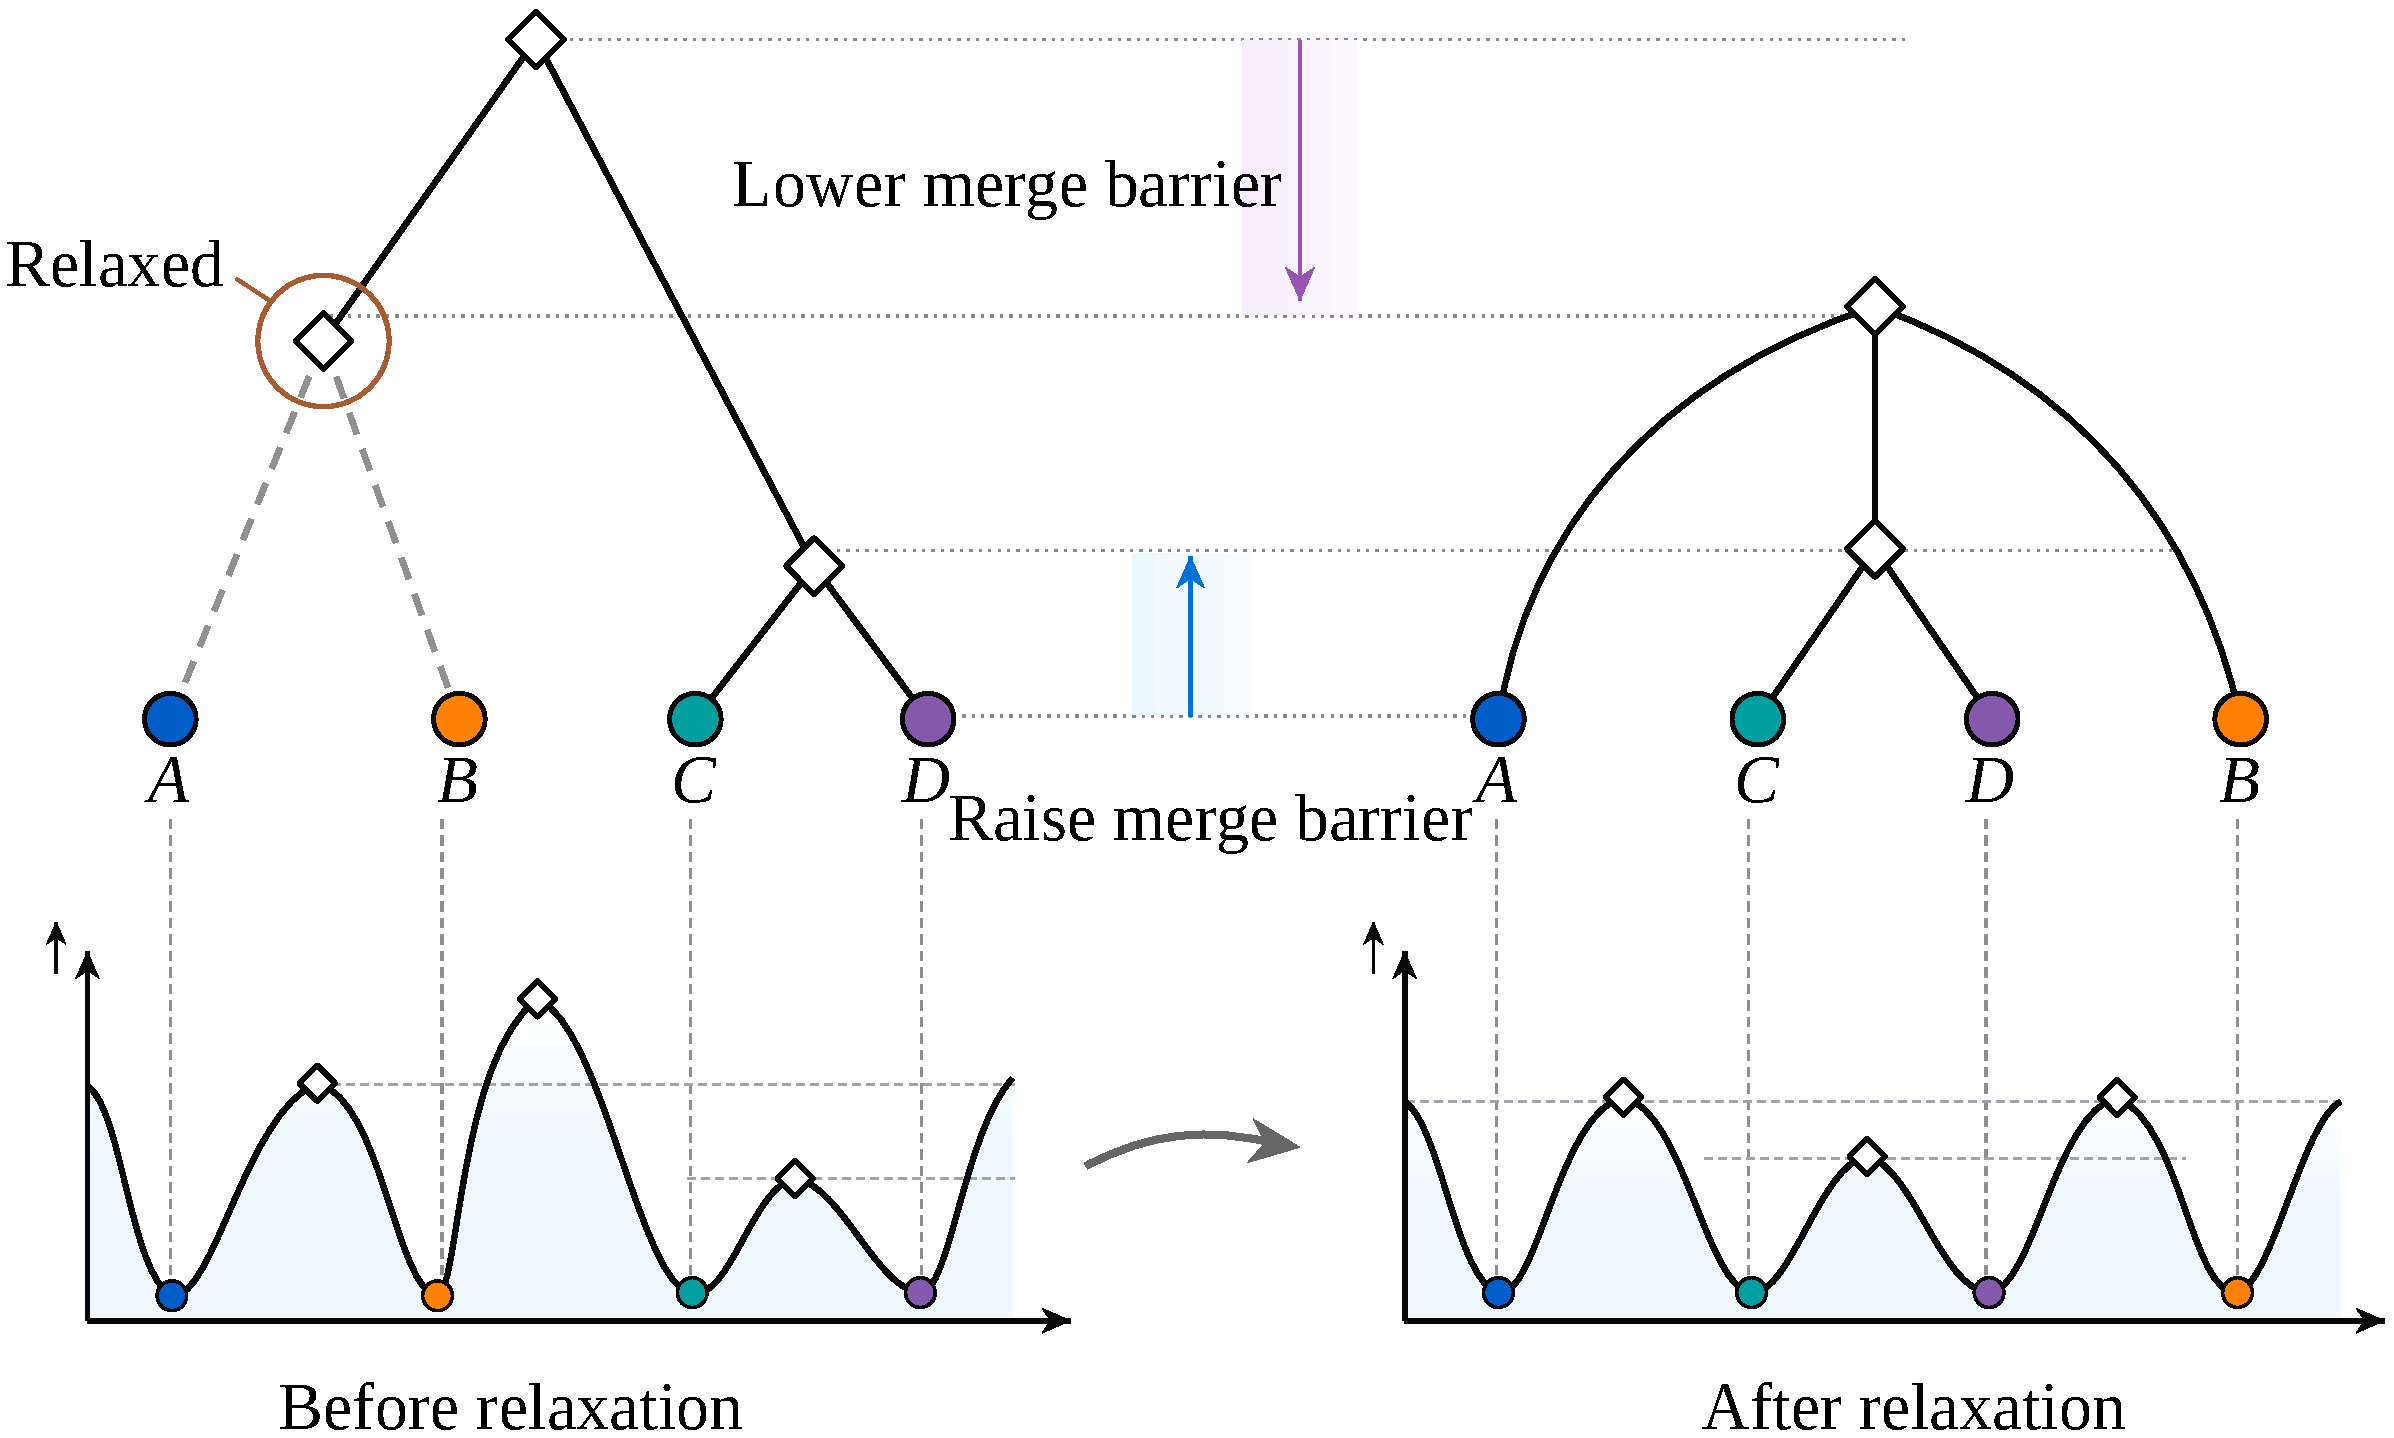
\includegraphics[width=\columnwidth]{figures/anchor_relaxation_open.pdf}
\caption{Selective flattening admits order $A,C,D,B$ while retaining the $C,D$ grouping. The displayed barrier levels are corrected against the original merge matrix.}
\label{fig:selective_relaxation}
\end{figure}
For gap $k$ of an order, set $C_k=\min_{i\le k<j}V_{\pi(i)\pi(j)}$ and let $F_k$ be the larger adjacent extremum value.
\begin{proposition}[Optimal barriers]\label{prop:barriers}
With fixed extrema, the least continuous merge error is
\begin{equation}\label{eq:delta}
\delta^*(\pi)=\max\Bigl\{0,\max_k(F_k-C_k),
\tfrac12\max_{i<j}\bigl(V_{\pi(i)\pi(j)}-\max_{i\le k<j}C_k\bigr)\Bigr\},
\end{equation}
attained by $b_k=C_k+\delta^*(\pi)$.
\end{proposition}
Indeed, error $\delta$ requires $F_k\le b_k\le C_k+\delta$; choosing the largest permitted barriers meets every pair's lower requirement exactly when $\delta\ge\delta^*$. This gives a closed-form admission test for candidate orders. Barriers equal to $F_k$ keep every label and extremum value but can flatten a basin; requiring a basin depth of at least $\gamma$ replaces $F_k$ by $F_k+\gamma$ in Eq.~\ref{eq:delta} by the same argument. Our admission test uses $F_k$ itself; Section~\ref{sec:reconstruction} gives the rendering clearance.

\subsection{Capped Spatiotemporal Placement}
For the chosen order, the default weights are $(\lambda_R,\lambda_G,\lambda_M,\lambda_C)=(4,1,0.5,0.1)$. Each term in Eq.~\ref{eq:family} is a mean squared residual: anchor-to-reference distance, ordered anchor separation minus support-centroid distance, matched temporal-target error, or anchor-to-center offset. The temporal target follows projected motion:
\begin{equation}\label{eq:temporal_target}
\hat x_i^t=x_{\mu_t(i)}^{t-1}+q_i^t-q_{\mu_t(i)}^{t-1}.
\end{equation}
The selected order is now fixed, so placement changes coordinates without revisiting the discrete search. Unmatched leaves have no temporal penalty. Placement solves the convex quadratic objective under the interval constraints and
\begin{equation}\label{eq:qp}
\|x-q\|_\infty\le\tau(\pi^\varepsilon)+\beta_0,
\end{equation}
with fixed slack $\beta_0$. Because $\tau$ is attained, this cap is feasible and transfers the selected order's displacement control to the final anchors. The cap prevents a relative-distance or temporal term from moving an anchor arbitrarily far from its spatial target. Within a frame the feasible set is linear and the objective quadratic; frame order enters only through matched predecessor targets.

\subsection{Profile Reconstruction}\label{sec:reconstruction}
The final stage receives the order, anchor intervals and optimal barriers. Leaf-arc samples fill the intervals and LCA paths fill their gaps~\cite{Koepp:2023:TMTM,STMTM:2026}. Barrier correction clips each inter-anchor interior to $b_k$ and raises its peak when needed. In every column that uses the budget, each barrier is raised to at least $F_k+10^{-6}(1+|F_k|)$, so every extremum stays a strict minimum. Profiles share direction, origin, extent and pixel scale; their stack is $I^\varepsilon(t,u)=\psi_t^\varepsilon(u)$. Rounding and this clearance can change merge levels, so the fixed-label matrix, including its diagonal, is rebuilt from every rendered column and its largest deviation from the tree is checked against $\eta$; this rendered error is the merge error we report. A frame that fails is recorded as a violation, not repaired or solved again, and a budget with any violation cannot be Balanced; no reported frame fails (Supplementary Section~S4.10).
\begin{table*}[!tb]
\caption{Comparison on five planar sequences (top) and two volumes (bottom). Bold/underline mark best/second distinct values among comparable local measurements only; ties share emphasis. Daggered SNS/TW values are published context and excluded from ranking. Curves use fixed default orientations.}
\label{tab:quantitative-final}
\footnotesize
\setlength{\tabcolsep}{1.5pt}
\renewcommand{\arraystretch}{0.85}
\begin{tabular*}{\textwidth}{@{\extracolsep{\fill}}l*{12}{c}lccc@{}}
\toprule
\multirow{2}{*}{Dataset} & \multicolumn{3}{c}{Hilbert} & \multicolumn{3}{c}{Morton} & \multicolumn{3}{c}{TMTM} & \multicolumn{3}{c}{ST-MTM} & \multicolumn{4}{c}{AnchorMTM (ours)} \\
\cmidrule(lr){2-4}\cmidrule(lr){5-7}\cmidrule(lr){8-10}\cmidrule(lr){11-13}\cmidrule(lr){14-17}
 & SNS$\downarrow$ & TW$\uparrow$ & NPE$\downarrow$ & SNS$\downarrow$ & TW$\uparrow$ & NPE$\downarrow$ & SNS$\downarrow$ & TW$\uparrow$ & NPE$\downarrow$ & SNS$\downarrow$ & TW$\uparrow$ & NPE$\downarrow$ & Mode & SNS$\downarrow$ & TW$\uparrow$ & NPE$\downarrow$ \\
\midrule
\multirow{2}{*}{Gaussian} & \multirow{2}{*}{$0.1117$} & \multirow{2}{*}{$0.6719$} & \multirow{2}{*}{$0.7557$} & \multirow{2}{*}{$\underline{0.0393}$} & \multirow{2}{*}{$\underline{0.8333}$} & \multirow{2}{*}{$0.7359$} & \multirow{2}{*}{$0.25^{\dagger}$} & \multirow{2}{*}{$0.77^{\dagger}$} & \multirow{2}{*}{$\underline{0.1118}$} & \multirow{2}{*}{$0.06^{\dagger}$} & \multirow{2}{*}{$1.00^{\dagger}$} & \multirow{2}{*}{$0.1154$} & Exact & $\mathbf{0.0353}$ & $\mathbf{0.9323}$ & $\mathbf{0.0089}$ \\
 &  &  &  &  &  &  &  &  &  &  &  &  & Balanced & $\mathbf{0.0353}$ & $\mathbf{0.9323}$ & $\mathbf{0.0089}$ \\
\multirow{2}{*}{Ring} & \multirow{2}{*}{$\mathbf{0.1252}$} & \multirow{2}{*}{$0.9048$} & \multirow{2}{*}{$0.5941$} & \multirow{2}{*}{$0.1489$} & \multirow{2}{*}{$0.7619$} & \multirow{2}{*}{$0.6033$} & \multirow{2}{*}{$0.28^{\dagger}$} & \multirow{2}{*}{$0.68^{\dagger}$} & \multirow{2}{*}{$0.1756$} & \multirow{2}{*}{$0.21^{\dagger}$} & \multirow{2}{*}{$0.88^{\dagger}$} & \multirow{2}{*}{$0.2463$} & Exact & $0.1485$ & $0.8571$ & $\underline{0.0471}$ \\
 &  &  &  &  &  &  &  &  &  &  &  &  & Balanced & $\underline{0.1334}$ & $0.8571$ & $\mathbf{0.0395}$ \\
\multirow{2}{*}{Wildfires} & \multirow{2}{*}{$0.1883$} & \multirow{2}{*}{$0.8303$} & \multirow{2}{*}{$0.3641$} & \multirow{2}{*}{$0.1304$} & \multirow{2}{*}{$0.8758$} & \multirow{2}{*}{$0.1560$} & \multirow{2}{*}{$0.44^{\dagger}$} & \multirow{2}{*}{$0.88^{\dagger}$} & \multirow{2}{*}{$0.2280$} & \multirow{2}{*}{$0.24^{\dagger}$} & \multirow{2}{*}{$0.91^{\dagger}$} & \multirow{2}{*}{$0.3180$} & Exact & $\mathbf{0.0426}$ & $0.9136$ & $\underline{0.0131}$ \\
 &  &  &  &  &  &  &  &  &  &  &  &  & Balanced & $\underline{0.0447}$ & $0.8989$ & $\mathbf{0.0116}$ \\
\multirow{2}{*}{Storms} & \multirow{2}{*}{$0.1290$} & \multirow{2}{*}{$0.7403$} & \multirow{2}{*}{$0.3705$} & \multirow{2}{*}{$0.1180$} & \multirow{2}{*}{$0.7251$} & \multirow{2}{*}{$0.3468$} & \multirow{2}{*}{$0.34^{\dagger}$} & \multirow{2}{*}{$0.71^{\dagger}$} & \multirow{2}{*}{$0.5753$} & \multirow{2}{*}{$0.21^{\dagger}$} & \multirow{2}{*}{$0.94^{\dagger}$} & \multirow{2}{*}{$0.4579$} & Exact & $\underline{0.0790}$ & $0.8463$ & $\underline{0.0399}$ \\
 &  &  &  &  &  &  &  &  &  &  &  &  & Balanced & $\mathbf{0.0743}$ & $0.8766$ & $\mathbf{0.0140}$ \\
\multirow{2}{*}{PM2.5} & \multirow{2}{*}{$0.2386$} & \multirow{2}{*}{$\mathbf{0.8887}$} & \multirow{2}{*}{$0.8090$} & \multirow{2}{*}{$\underline{0.1760}$} & \multirow{2}{*}{$\underline{0.8277}$} & \multirow{2}{*}{$0.8823$} & \multirow{2}{*}{$0.3018$} & \multirow{2}{*}{$0.7781$} & \multirow{2}{*}{$0.5241$} & \multirow{2}{*}{$0.1897$} & \multirow{2}{*}{$0.8224$} & \multirow{2}{*}{$0.5577$} & Exact & $0.1964$ & $0.7884$ & $\underline{0.1390}$ \\
 &  &  &  &  &  &  &  &  &  &  &  &  & Balanced & $\mathbf{0.1636}$ & $0.7657$ & $\mathbf{0.0468}$ \\
\midrule
\multirow{2}{*}{Cylinder} & \multirow{2}{*}{$0.2798$} & \multirow{2}{*}{$0.7902$} & \multirow{2}{*}{$0.3700$} & \multirow{2}{*}{$0.2071$} & \multirow{2}{*}{$0.8008$} & \multirow{2}{*}{$0.2810$} & \multirow{2}{*}{$0.2956$} & \multirow{2}{*}{$0.8017$} & \multirow{2}{*}{$0.4769$} & \multirow{2}{*}{$0.1346$} & \multirow{2}{*}{$\underline{0.8989}$} & \multirow{2}{*}{$0.5160$} & Exact & $\underline{0.1097}$ & $0.8136$ & $\underline{0.0918}$ \\
 & & & & & & & & & & & & & Balanced & $\mathbf{0.0405}$ & $\mathbf{0.8998}$ & $\mathbf{0.0133}$ \\
\multirow{2}{*}{Tangaroa} & \multirow{2}{*}{$0.3429$} & \multirow{2}{*}{$\mathbf{0.9222}$} & \multirow{2}{*}{$0.2646$} & \multirow{2}{*}{$0.3627$} & \multirow{2}{*}{$\underline{0.8893}$} & \multirow{2}{*}{$0.4486$} & \multirow{2}{*}{$0.5255$} & \multirow{2}{*}{$0.6701$} & \multirow{2}{*}{$0.3866$} & \multirow{2}{*}{$0.1655$} & \multirow{2}{*}{$0.8137$} & \multirow{2}{*}{$0.3286$} & Exact & $\underline{0.1518}$ & $0.8061$ & $\underline{0.0861}$ \\
 & & & & & & & & & & & & & Balanced & $\mathbf{0.1364}$ & $0.8476$ & $\mathbf{0.0465}$ \\
\bottomrule
\end{tabular*}
\vspace{2pt}
\begin{minipage}{\textwidth}\footnotesize For the original four inputs, TMTM/ST-MTM Temporal SNS/TW ($\dagger$) are published values; other entries are local measurements. The four inputs are our reconstructions (Section~\ref{sec:experiments}). TW needs enough features per frame: 64/64, 1/40, 4/32 and 11/744 frames are eligible on Gaussian, Ring, Wildfires and Storms, so TW is not ranked on the last three. Published TW has two-decimal precision. Mode applies only to AnchorMTM. PM2.5 uses 744 shared-input local frames (TW $k=1$, full coverage); its Balanced mode uses the fixed exploratory 5\% case budget, without validation-set budget selection. ST-MTM uses the Storms preset with start frame 0; PM2.5 baseline metrics are all recomputed. Volumes: all entries local, streamwise $x$ reference, TW $k=1$; Balanced is 1\% (Cylinder) and 9\% (Tangaroa) by the planar rule, attaining 0.99\% and 9.0\% merge error. ST-MTM was not proposed for volumes; its volume rows are our adaptation (Section~\ref{sec:experiments}).\end{minipage}

\end{table*}


\section{Evaluation}\label{sec:experiments}
The evaluation follows the argument of the paper. We first test the bounds and use them to measure how much of the error of existing maps the tree actually forces; this evidence does not depend on what AnchorMTM optimizes. We then ask whether the anchored axis reaches its goal and what that costs in relative geometry and temporal behavior, examine how a merge budget changes individual frames, and read an anchored map against its source field.

\subsection{Data and Measures}
\paragraph{Data.} The four planar sequences are Ring (40 frames), Wildfires (32) and Storms (744), our reconstructions of the ST-MTM benchmark~\cite{STMTM:2026} at its per-frame persistence fractions, because its processed arrays are not available, and hourly PM$_{2.5}$ over northern China in January 2017 (744 frames, 5\% persistence)~\cite{Kong:2021:CAQRA}; Storms uses ERA5 sea-level-pressure anomalies~\cite{Hersbach:2020:ERA5} and Wildfires aggregated fire radiative power~\cite{Franke:2021:1DP}. We omit the Gaussian sequence of that benchmark, which has three features per frame and no conflict between hierarchy and position. The volumes are the flow past a square cylinder (102 frames of the $Q$-criterion, 2\% persistence)~\cite{Camarri:2005:Cylinder,Weinkauf:SquareCylinder} and the Tangaroa ship wake (201 speed fields, absolute persistence 0.2)~\cite{Popinet:2004:Tangaroa}. Within each comparison, all methods share the fields, trees, identities and references.

\paragraph{Compared maps.} TMTM and ST-MTM keep the tree but define no origin or direction for their axis, so each is reflected once per sequence to agree with the reference. ST-MTM was proposed for planar data, and its authors make no claim about volumes; because it is the only existing map that optimizes relative geometry and its inputs do not depend on the dimension, we include our own 3-D adaptation, with 3-D distances and the method's general parameters and without tuning (Supplementary Section~S4.2). Its volume rows report this adaptation, not a result of its authors. The Hilbert and Morton space-filling curves are references for neighborhood quality only: they order all samples of the domain and break the tree, and a curve index corresponds to no spatial direction, so we report no NPE for them and do not rank them.

\paragraph{Measures.} Table~\ref{tab:measures} lists the measures. NPE is our own: AnchorMTM optimizes it and TMTM and ST-MTM do not, so it shows whether the anchoring goal is reached and does not rank the maps in general. The bound and the measures from prior work do not depend on it. SNS and TW compare anchor distances with support-centroid distances; for the three benchmark inputs, the published TMTM and ST-MTM values are quoted for context (daggers in Table~\ref{tab:quantitative-final}). TW needs enough features per frame and is not ranked on Ring, Wildfires and Storms, where only 1, 4 and 11 frames are eligible.

\begin{table}[!tb]
\centering
\caption{Measures of the evaluation. Lower is better, except for TW (higher) and TD (no preferred value, since features do move).}
\label{tab:measures}
\footnotesize
\setlength{\tabcolsep}{3pt}
\renewcommand{\arraystretch}{0.95}
\begin{tabular}{@{}lp{.68\columnwidth}l@{}}
\toprule
Measure & Meaning & Source\\
\midrule
$\nu^*$ & Smallest order error the tree forces (Eq.~\ref{eq:nu}) & this paper\\
NROE & Order error: least worst displacement of a leaf order (Eq.~\ref{eq:nroe}) & this paper\\
NPE & Worst displacement of the drawn map (Eq.~\ref{eq:nroe}) & this paper\\
Merge & Largest change of a displayed merge level (Eq.~\ref{eq:dtop}) & \cite{Munch:2019:LINF}\\
SNS & Scale-normalized stress of distances & \cite{Smelser:2025:Scale}\\
TW & Trustworthiness of neighbors & \cite{Venna:2001:NP}\\
TD & Summed displayed motion of matched anchors & \cite{STMTM:2026}\\
ME & Share of feature pairs whose displayed approach or separation contradicts the true one & --\\
\bottomrule
\end{tabular}
\end{table}

\paragraph{Modes.} Exact uses zero allowance. Balanced uses a positive budget selected once from 1--10\% on the first chronological quarter of each benchmark input (1, 5 and 10\%); PM$_{2.5}$ uses a fixed 5\%. The volumes use the default configuration, the same Balanced rule and the streamwise axis of both flows as a supplied direction (Section~\ref{sec:reference-model}; Supplementary Section~S4.7 gives Tangaroa along its motion); Table~S1 lists the other settings.

\begin{figure*}[!tb]
\centering
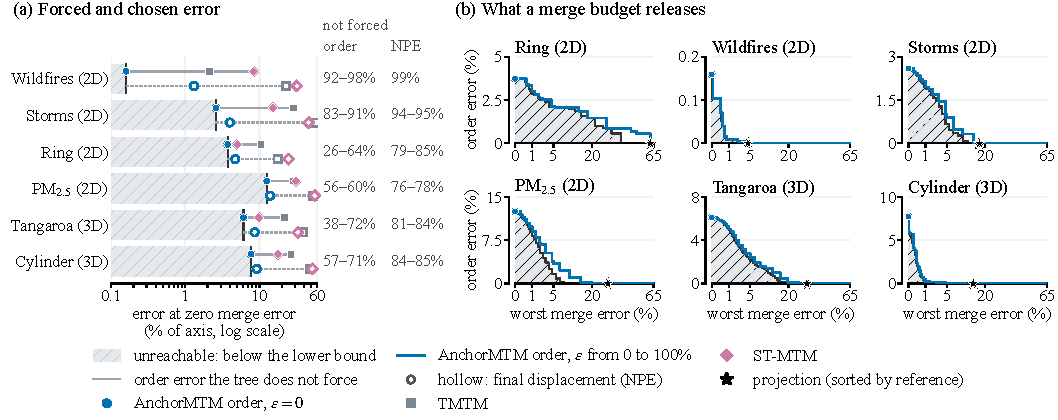
\includegraphics[width=\textwidth]{figures/forced_plane.pdf}
\caption{Forced and chosen error. (a)~The steps of Section~\ref{sec:bounds} for maps that keep the tree (log scale). The hatched region is what the tree forces: no exact map can lie below the bound $\nu^*$. Filled markers are the order error of each map, hollow markers its final displacement NPE. Midpoint ordering (blue, filled) lies on the bound; TMTM and ST-MTM lie far above it. The right columns give the share of TMTM and ST-MTM error above the bound. (b)~The bound as the merge error grows (Proposition~\ref{thm:chain} and the flattened bound), each panel scaled to its own bound. The budgeted point-model order of AnchorMTM ($\varepsilon$ from 0 to 100\%; worst merge error on a square-root scale) runs along it; the projection keeps every reference but breaks the tree.}
\label{fig:plane}
\end{figure*}
\begin{figure*}[!tb]
\paperfigure[\textwidth]{figures/volume_gallery.pdf}{fig:volume-gallery}{Where each map draws the features of Tangaroa and Cylinder along the streamwise axis; the TMTM, ST-MTM and $\varepsilon=0$ columns are the runs of Table~\ref{tab:quantitative-final}. The first column is the reference $q$, the actual location of each feature along $a^*$ and the target of the comparison; light grey dots repeat it in the other panels, and color shows how far a feature is drawn from it. The bars give NPE, the worst displacement of a frame averaged over frames (\% of the axis); for positive budgets, the value in parentheses is the merge error, the largest change of any displayed merge level (\% of the scalar range), a magnitude and not an error rate. TMTM, ST-MTM and $\varepsilon=0$ show the tree exactly. Each baseline is reflected once to reduce its displacement.}
\end{figure*}
\subsection{Tightness of the Bounds and Forced Error}\label{sec:bounds-eval}
\emph{Controlled trees.} On two sibling pairs below a root, minimax linear programs over all 24 leaf orders, the width-aware bound and the selected order coincide at all 43 overlaps, and all 364 budget tests release the conflict exactly at $2\varepsilon=h$, as Proposition~\ref{thm:chain} predicts.

\emph{Real trees.} The selected Exact order attains the width-aware bound on 1,271 of 1,560 planar frames, so on these frames no exact-topology order has a smaller worst displacement. Ring attains it on every frame, Wildfires misses one frame and Storms 15. PM$_{2.5}$ attains it on 471 of 744 frames and leaves a small residual gap: the mean interval cost is 13.11\% of the axis against a mean bound of 12.88\%. We did not evaluate width-aware attainment on the volumes.

\emph{Forced and chosen error.} Bounds are evaluated at the numerical tolerance $\varepsilon_0$ of Section~\ref{sec:method}, as the maps are; this matters only on Cylinder, where near-equal merge levels in 34 of 102 frames lower the mean $\nu^*$ from 12.2\% to 7.7\%. Figure~\ref{fig:plane}a reads the steps of Section~\ref{sec:bounds} for each map. Midpoint ordering attains $\nu^*$ on the same tree, so the step from $\nu^*$ to the order error is chosen by the order rule. On the real-data sequences, 83--98\% of the order error of TMTM and ST-MTM on Wildfires and Storms and 56--60\% on PM$_{2.5}$ lie above $\nu^*$ and could be removed without changing the tree; on the two volumes it is 38--72\%, and on the synthetic Ring 26--64\%. The step from order error to NPE comes from packing and placement: measured in NPE, 76--99\% of the error of TMTM and ST-MTM lies above $\nu^*$. The bounds also reveal how strongly a field entangles its hierarchy with space: $\nu^*$ is 0.16\% of the axis on Wildfires and 2.6\% on Storms, but 12.5\% on PM$_{2.5}$, where nested pollution maxima interleave along the chosen direction. The bound under a merge budget shows what a budget releases (Fig.~\ref{fig:plane}b). Where conflicting subtrees merge just below their parent, little is needed: 1\% removes almost all forced order error on Wildfires (0.16\% to 0.01\%) and on Cylinder (7.7\% to 0.2\%). Where conflicts lie deep, position is expensive: PM$_{2.5}$ needs 10\% to fall below 1\%, and Tangaroa 12\%. The projection reaches zero order error only by changing merge levels by 4--62\% of the scalar range.

\subsection{Position and What It Costs}\label{sec:reference-results}
\emph{Position.} NPE tells whether the anchored axis reaches its goal. With zero merge error, Exact lowers NPE relative to TMTM and ST-MTM by 73--96\% on all four planar inputs, from 48--52\% to 9.2\% on Cylinder and from 33--39\% to 8.6\% on Tangaroa (Table~\ref{tab:quantitative-final}). Balanced, with a budget of at most 10\%, lowers it further on every input. Giving the baselines their best affine map of the axis per sequence, which favors them, still leaves 28--33\% on Tangaroa and 45\% on Cylinder. In Fig.~\ref{fig:volume-gallery}, TMTM and ST-MTM place the features of both volumes in bands that do not follow the references, whereas Exact already reproduces the shedding pattern of Cylinder, and a 5\% budget removes almost all of the rest (NPE 1.2\%). Because AnchorMTM optimizes NPE, these results show that the goal is reached, not that AnchorMTM is better in general; the next two paragraphs use measures that do not depend on it.

\emph{Relative geometry.} SNS and TW measure the goal of ST-MTM. With the tree kept exactly, ST-MTM keeps the higher TW wherever every score is measured locally (PM$_{2.5}$ and both volumes); Exact has the lower SNS on both volumes, ST-MTM on PM$_{2.5}$. With a budget, Balanced improves on ST-MTM in both SNS and TW on both volumes, narrowly in TW on Cylinder (0.8998 against 0.8989), and in SNS on PM$_{2.5}$ (Table~\ref{tab:quantitative-final}). The higher TW at exact topology follows from what ST-MTM optimizes, not from a weaker pipeline: ST-MTM is another setting of Eq.~\ref{eq:family}. Giving our placement the leaf order of the ST-MTM run, $\lambda_R=0$, no position cap and a stationary temporal target yields SNS and TW of 0.1419 and 0.8925 on Cylinder and of 0.1439 and 0.8349 on Tangaroa, with NPE back at 48\% and 29\% (Supplementary Section~S4.5). A map that drew every feature exactly at its reference would have TW 0.862 on Cylinder and 0.763 on Tangaroa, below ST-MTM: one spatial axis cannot keep the neighbors of a 2-D or 3-D field, as on all seven sequences we tested (Supplementary Table~S3). As references, the curves reach a lower SNS on Ring (Hilbert 0.1252 against 0.1334) and a higher TW on PM$_{2.5}$ and Tangaroa (Hilbert 0.8887 and 0.9222), at the price of the tree.

\emph{Temporal behavior.} TD is small for a map that holds features still. On Cylinder, Exact has TD 57 against 43 for ST-MTM. Part of this is real motion, since drawing the references themselves gives 27; the rest comes from leaf-order changes between frames, which a 10\% budget reduces to 29. On Tangaroa, Exact moves less than ST-MTM (107 against 139). Motion errors (ME) are fewer for Exact than for TMTM and ST-MTM on all seven sequences (33\% against 46--67\% on Cylinder, 59\% against 70--97\% on Tangaroa).

\begin{figure*}[!tb]
\centering
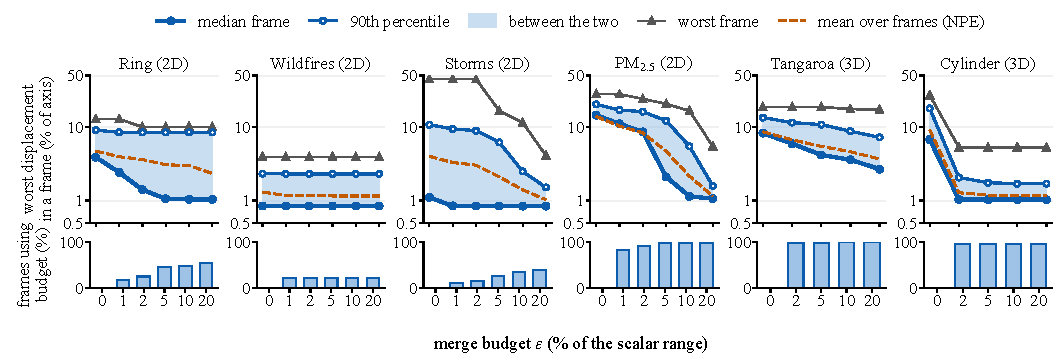
\includegraphics[width=\textwidth]{figures/budget_response_v30.pdf}
\caption{How a merge budget acts across frames. For each sequence and budget, the worst displacement of every frame is summarized over all frames: the median frame, the 90th percentile and the worst frame (log scale), and the mean over frames, which is NPE (dashed). Bottom: the share of frames whose attained merge error is positive, that is, frames that use the budget. Every frame stays within its budget. The volumes were not run at 1\%.}
\label{fig:budget-distribution}
\end{figure*}
\subsection{How a Merge Budget Acts across Frames}\label{sec:relaxation-results}
A budget limits merge error, not displacement, so its effect depends on how many frames contain a conflict it can release (Fig.~\ref{fig:budget-distribution}). Two regimes appear. On Storms the budget acts on a tail: 35\% of the frames use the allowance at $\varepsilon=10\%$, the median displacement moves only from 1.10\% to 0.84\%, but the 90th percentile falls from 10.7\% to 2.5\% and the worst frame from 44.8\% to 11.6\%. On PM$_{2.5}$ and the volumes almost every frame contains a releasable conflict and the whole distribution moves: on PM$_{2.5}$, 97\% of the frames use a 5\% budget and the median falls from 14.5\% to 2.1\%; on Cylinder, 2\% already lowers the median from 6.8\% to 1.0\%; on Tangaroa the median falls from 8.2\% to 3.6\% at 10\% and to 2.7\% at 20\%. The share of frames that use the budget is thus itself a diagnostic of how strongly a sequence entangles hierarchy and space. Exact has zero merge error on every input; Balanced attains at most 0.982, 4.421 and 9.985\% on Ring, Wildfires and Storms, and every frame passes the continuous and raster checks. Supplementary Fig.~S4 samples the budget more finely.

\begin{figure*}[!tb]
\centering
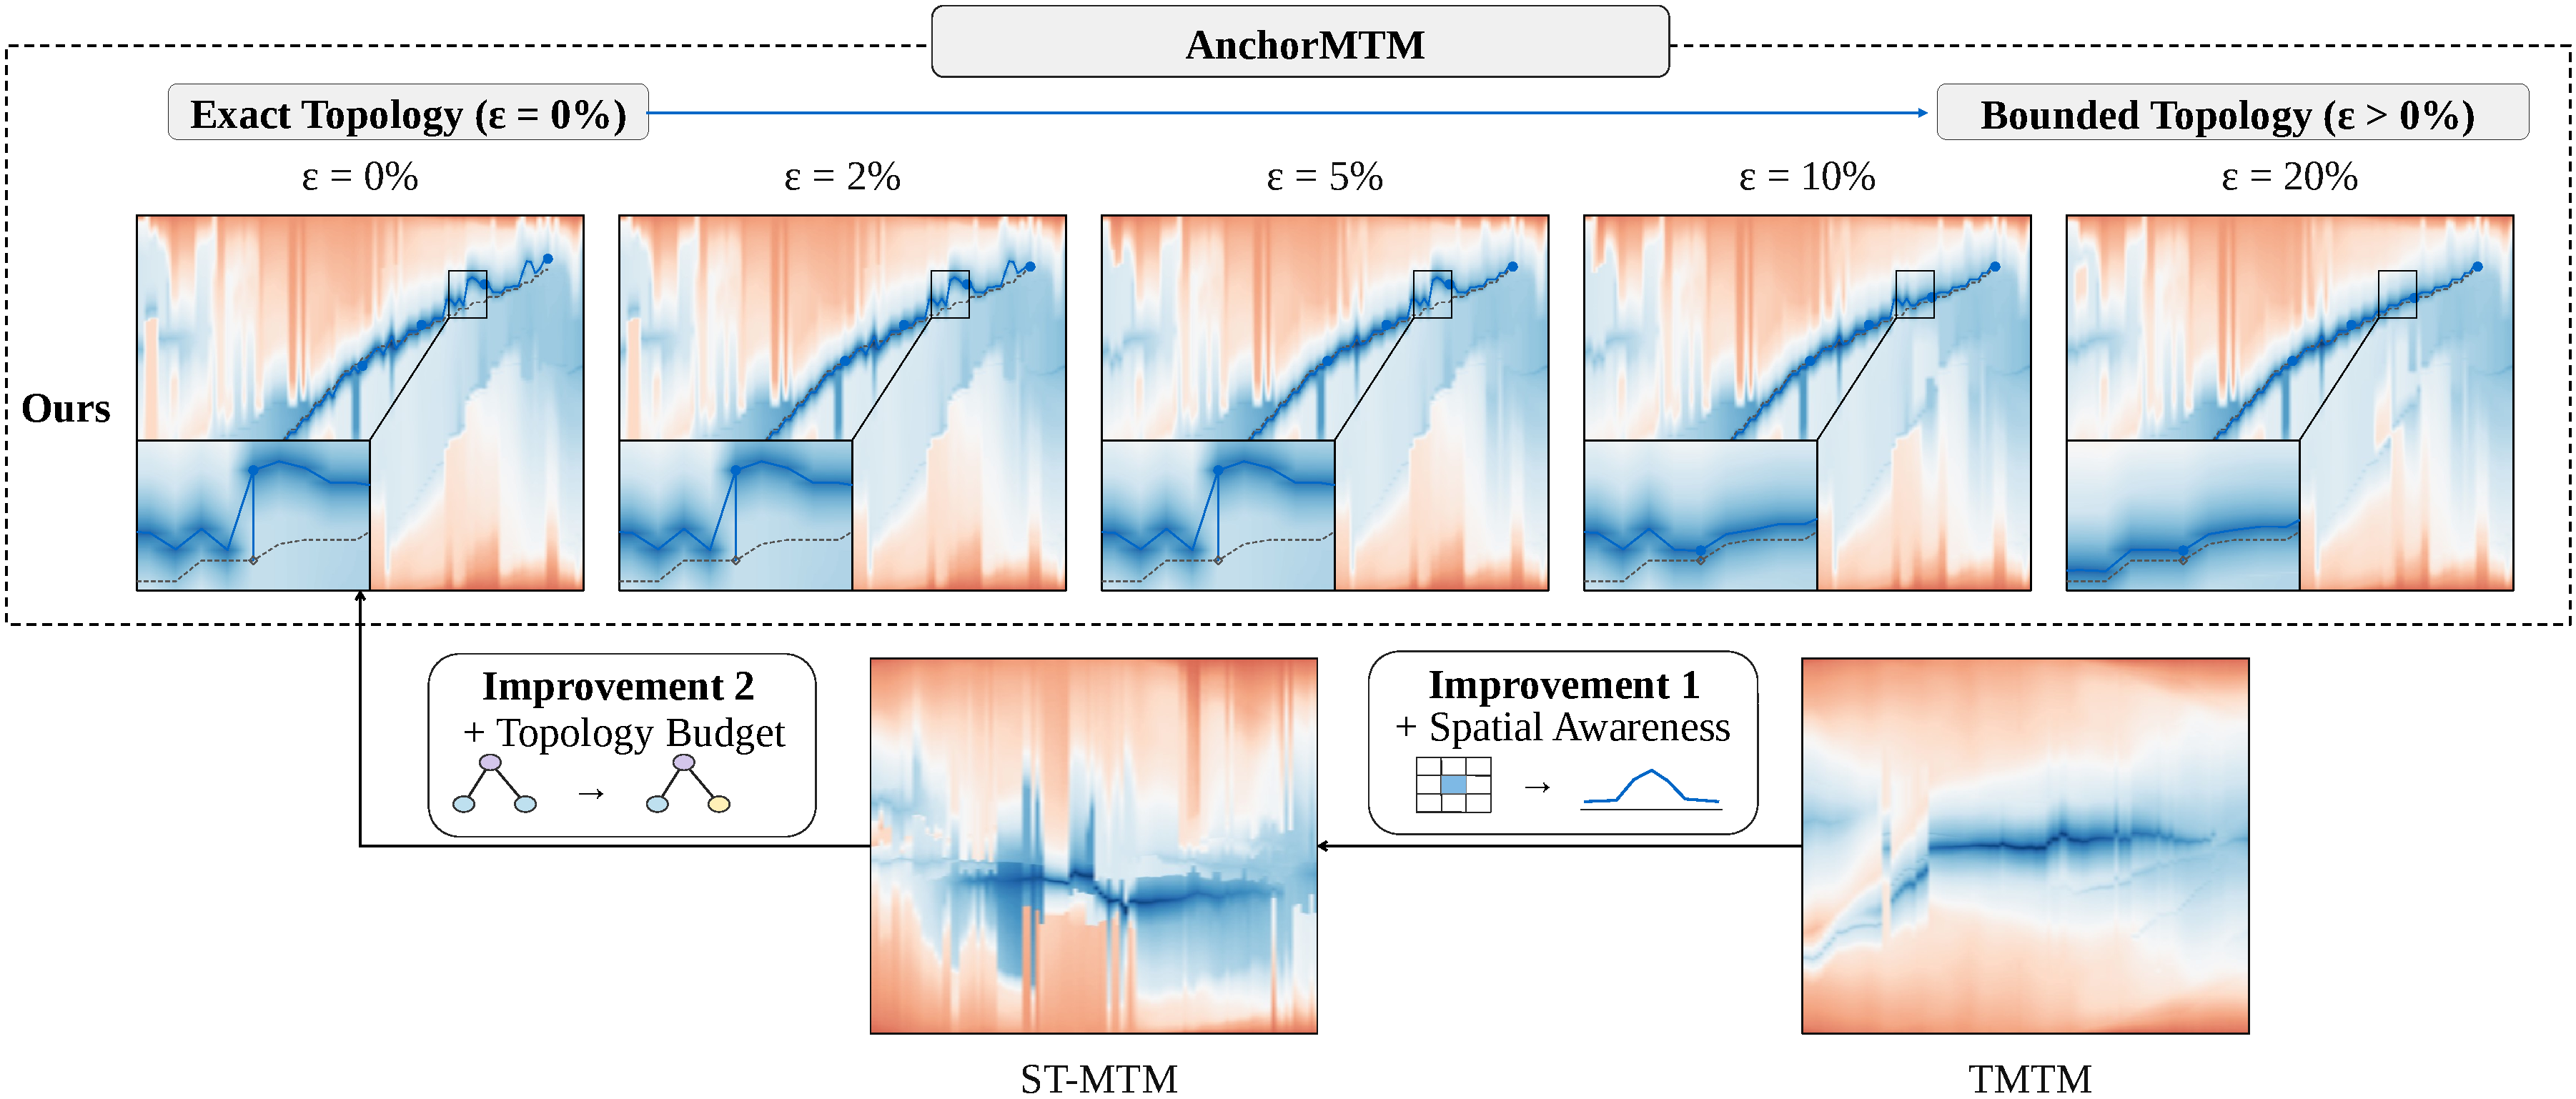
\includegraphics[width=\textwidth]{figures/anchor_storms_budget_maps.pdf}
\caption{Storms event window, frames 355--460, drawn by AnchorMTM at five budgets and by TMTM and ST-MTM on the same fields and trees, on one $[-35,35]$\,hPa scale. The lower comparison illustrates two improvements: ST-MTM adds pairwise spatial distances to TMTM's tree order, and AnchorMTM gives the axis one fixed direction and controls the merge levels it may change. The dashed curve in the insets is the reference trajectory of the tracked storm.}
\label{fig:storms-budget-profiles}
\end{figure*}
\subsection{Reading Anchored Maps}\label{sec:case-studies}
\paragraph{A storm crossing the North Atlantic.} Figures~\ref{fig:storms_overview} and~\ref{fig:storms-budget-profiles} follow one low from the open Atlantic to Scandinavia between 16 and 19 December 1999. In the AnchorMTM maps its band rises steadily along the axis, and the rise is the storm's eastward motion, while the profile still shows how it merges with the neighboring lows. TMTM aligns subtrees by temporal overlap and ST-MTM places them by relative distance, so both keep the storm near the same height and its motion cannot be read from the map. The budget changes the picture locally: at 0, 2 and 5\% the maps coincide in this window, while 10 and 20\% release the remaining conflict and move the storm onto its reference trajectory (insets).

\paragraph{Vortex shedding behind a cylinder.} The anchored default places the shed vortices at their streamwise positions (Fig.~\ref{fig:volume-gallery}). When the wake changes regime is read better if the hierarchy is given priority: an exploratory variant that freezes the leaf order of a compact TMTM layout and guides the anchors toward it separates five stages of the wake, but gives up the spatial axis (Supplementary Section~S4.8). The two readings complement each other. Supplementary Fig.~S7 reads an hourly PM$_{2.5}$ episode in the three maps.

\subsection{Implementation and Verification}
Each rendered column is checked against the fixed-label merge matrix of its source tree, together with interval order, capacity, gaps and anchor slack, and the bounds and baseline inversion errors are recomputed independently (Supplementary Section~S4.10). Ordering and placement take 0.15--3.32\,s per benchmark sequence and 200\,s for the 744-frame PM$_{2.5}$ sequence on an Apple M4 (Supplementary Table~S1).

\section{Discussion}\label{sec:discussion}
\paragraph{What the bound reveals about the data.} The exact-topology bound is a property of a field and a direction, not of a layout, and it is informative on its own. A small $\nu^*$, as on Wildfires and Storms, says that the hierarchy of the field and its geography largely agree: sibling subtrees occupy separate stretches of the axis, and any good order can draw features near their locations. A large $\nu^*$, as on hourly PM$_{2.5}$, says that nested maxima interleave in space; there, a map that keeps the tree must displace features, and the displacement measures how far the merge structure of the field departs from its spatial arrangement. Because the bound requires no layout, it can be computed for several candidate directions before a map is drawn and used to choose the axis along which hierarchy and space conflict least.

\paragraph{Forced error versus layout choice.} The gap between existing maps and the bound is the most practical finding. Most of the order error of TMTM and ST-MTM on our real-data sequences is not forced by the tree; it follows from ordering leaves without a spatial reference. Any merge tree map that keeps the tree, including future ones, can be measured against the same bound and judged on how much of its displacement it chooses.

\paragraph{Spending topological fidelity deliberately.} A merge budget changes merge levels by a declared amount; it never removes a feature, alters an extremum value or moves the data. Persistence simplification at a comparable threshold would delete features below it instead. The per-frame records show where the budget was spent, and the share of frames that use it distinguishes sequences whose conflicts are rare and deep, such as Storms, from sequences in which nearly every frame is entangled, such as PM$_{2.5}$ and the volumes. Marking the changed barriers in the map can keep this trade visible to the reader.

\paragraph{One axis, several readings.} A fixed spatial axis and a geometry-oriented embedding answer different questions. AnchorMTM supports reading position and motion along a chosen direction, ST-MTM preserves local neighborhoods better, and the central-tree variant of Fig.~\ref{fig:cylinder-centered} exposes regime changes. These readings complement one another, and a view that links them, or small multiples along several directions, could serve analysts who need more than one.

\paragraph{Limitations and future work.} AnchorMTM encodes one spatial direction; positions across it, and the full two- or three-dimensional geometry, are not shown on the axis. We plan to extend the bounds from one axis to a complete account of the fidelities a temporal map trades against one another, including position along several directions, temporal coherence and relative geometry, each with its own certificate. The default direction is estimated from the whole sequence, so streaming data need a direction chosen in advance. The order search is heuristic: it attains the width-aware bound on most planar frames but leaves a residual gap on PM$_{2.5}$ and on large volumetric trees. Finally, we have not yet measured how accurately analysts read position, motion and nesting from these maps; a controlled user study is the next step.

\section{Conclusion}\label{sec:conclusion}
We presented AnchorMTM, a merge tree map whose vertical axis is one fixed spatial direction, so that an analyst can read where features are and how they move while seeing how they nest. Keeping the merge tree and keeping location conflict, and we addressed this conflict in three steps: we formulated the construction of a spatially anchored map as one layout problem under a declared merge-error limit; we derived three lower bounds on the displacement that the tree forces, for exact topology, finite widths and bounded merge error; and we built the map from the data with a budgeted leaf-order search, optimal merge barriers and a capped placement. On five planar and two volumetric sequences, the selected orders attained the width-aware bound on 1,335 of 1,624 planar frames, most of the order error of existing maps proved not forced by the tree, and at the same exact topology AnchorMTM lowered the mean worst displacement by 73--96\%. Because the bounds depend only on the data, they tell before a map is drawn how much a spatial axis costs, where in the tree that cost arises, and how much merge-level fidelity buys it back. This turns the trade-off between topology and position into a quantity that can be measured and chosen, and it lays a foundation for temporal maps that certify several fidelities at once.

\FloatBarrier
\begingroup
\interlinepenalty=10000
\bibliographystyle{abbrv-doi-narrow}
\bibliography{references}
\endgroup
\end{document}
